\documentclass[aspectratio=169]{beamer}
\usetheme{default}
\usecolortheme{default}
\setbeamertemplate{navigation symbols}{}
\setbeamertemplate{footline}[frame number]
\usepackage{graphicx}
\usepackage{booktabs}
\usepackage{amsmath}
\usepackage{amssymb}
\usepackage{array}
\usepackage{xcolor}
\usepackage{multirow}

\definecolor{iasblue}{RGB}{23,55,110}
\definecolor{iasred}{RGB}{180,30,30}
\definecolor{iasgray}{RGB}{100,100,100}

\graphicspath{{figures/}}

% Table file compatibility: silence \begin{table} floats, \caption, \label
\makeatletter
\AtBeginDocument{%
  \renewenvironment{table}[1][]%
    {\par\begingroup\centering}%
    {\endgroup\par}%
  \def\caption{\@ifnextchar[\@caption@eat\@gobble}%
  \def\@caption@eat[#1]#2{\ignorespaces}%
  \renewcommand{\label}[1]{}%
}%
\makeatother

\title{Do Diplomas Deliver?}
\subtitle{Bureaucrat Education and Public Service Outcomes}
\author{Arya Gadage}
\date{May 29, 2026\\ PER Pre-Doctoral Mini Conference}

\begin{document}

\begin{frame}
\titlepage
\end{frame}

% -------------------------------------------------------
\begin{frame}{Outline}
\tableofcontents
\end{frame}

% ===============================================================
\section{Motivation}
% ===============================================================

\begin{frame}{The Paper}
\bigskip
\begin{itemize}
\item Indian Civil Service follows Macaulayan legacy $\rightarrow$  assigns bureaucrats to districts without accounting for programmatic fit.
\item Generalist ideals $\rightarrow$  An engineer or social scientist bureaucrat occupy identical roles, albeit face systematically different tasks depending on which programs dominate the district.
\item Educational training creates task-specific comparative advantage within a generalist bureaucracy, and whether the mismatch between officer type and program type has measurable costs.
\end{itemize}
\bigskip
\textbf{Research question:} Does the educational background of the District Collector affect which public goods get delivered, and how well?

\bigskip
\textbf{Policy margin:} Unlike selection quality or incentive design, posting rules are a zero-cost margin. Reweighting assignments by educational background costs nothing.

\end{frame}

% -------------------------------------------------------
% CHANGE 1: Added three new bullets + updated "This paper" bullet
\begin{frame}{Related Literature}

\begin{itemize}\setlength\itemsep{10pt}
  \item \textbf{Bureaucrat quality \& public goods delivery}\\
        {\small Finan, Olken \& Pande (2017); Dal~B\'o, Finan \& Rossi (2013);
        Rasul \& Rogger (2018); Bertrand, Burgess \& Xu (2020)}

  \item \textbf{Political economy of postings}\\
        {\small Iyer \& Mani (2012); Xu, Bertrand \& Burgess (2018)}

  \item \textbf{Comparative advantage \& assignment}\\
        {\small Roy (1951); Heckman \& Sedlacek (1985)}

  \item \textbf{Priority mechanisms \& matching theory}\\
        {\small Abdulkadiro\u{g}lu \& S\"onmez (2003);
        Roth \& Sotomayor (1990)}

  \item \textbf{Misallocation of resources}\\
        {\small Hsieh \& Klenow (2009)}

  \item \textbf{This paper:} first to exploit IAS educational background
        as a priority-queue instrument --- motivating optimal reallocation design
\end{itemize}
\end{frame}

% ===============================================================
\section{Institutional Setting}
% ===============================================================

\begin{frame}{The IAS and the District Collector}

\textbf{Indian Administrative Service:}
\begin{itemize}
    \item Recruited nationally via CSE (UPSC) competitive examination
    \item Allocated to state cadres for life (caste-based quotas + home preference)
    \item Generalist by design --- officers rotate across portfolios every 1--3 years
    \item Approximately 5,000 active officers; roughly 640 districts across India
\end{itemize}

\bigskip

\textbf{District Collector / District Magistrate:}
\begin{itemize}
    \item Principal administrative officer in a district; responsible for all program implementation
    \item Oversees PMGSY (rural roads), NREGA (welfare employment), electrification, land administration
    \item Posting determined by state government: seniority, vacancy, and political context
    \item No formal rule links educational background to district assignment
    \item Mean tenure $\approx$ 15--18 months (Iyer \& Mani 2012; consistent with our data)
\end{itemize}

\end{frame}
% ===============================================================
\section{Data}
% ===============================================================

\begin{frame}{Data}

\begin{itemize}
    \item \textbf{IAS administrative records} (Trivedi Center): DC posting spells for 4,348 officers, 1985--2008; designation, office, start/end dates, educational degree, cadre, allotment year

    \medskip

    \item \textbf{DMSP nightlights} (NOAA): Annual satellite-derived calibrated light output, all 640 Census 2011 districts, 1994--2008; fully observed, no missing values

    \medskip

    \item \textbf{PMGSY roads} (Ministry of Rural Development): Annual district rural road completions (km); coverage expands from 36 districts in 2001 to $\sim$340 by 2002--2008; restricted to 2001--2008

    \medskip

    \item \textbf{Economic Census employment} (MoSPI): Annual non-farm establishment employment, 553--640 districts; to isolate post-NREGA period

    \medskip

    \item \textbf{Census 2011} (RGI): SC/ST population share, literacy rate, total population; time-invariant controls absorbed by district fixed effects
\end{itemize}

\end{frame}
% -------------------------------------------------------
\begin{frame}{Educational Composition of DC Officers}

\begin{columns}[T]
\begin{column}{0.44\textwidth}
\vspace{0.3em}
{\small
\begin{tabular}{lrr}
\toprule
Group & Spells & Share \\
\midrule
Social Scientist & 873 & 36.8\% \\
Engineer         & 486 & 12.2\% \\
Residual         & 528 & 22.2\% \\
Unclassified     & 870 & 28.8\% \\
\midrule
Total (classified) & 1,887 & \\
\bottomrule
\end{tabular}
}

\vspace{0.8em}
{\footnotesize
Engineer: Engineering, Technology \& Mathematics.\\[2pt]
Social Scientist: Social Science, Liberal Arts, Governance \& Law.\\[2pt]
Residual: Natural Sciences, Medical.\\[2pt]
Unclassified: N.A.\ or missing education record.
}
\end{column}

\begin{column}{0.52\textwidth}

\begin{figure}
    \centering
    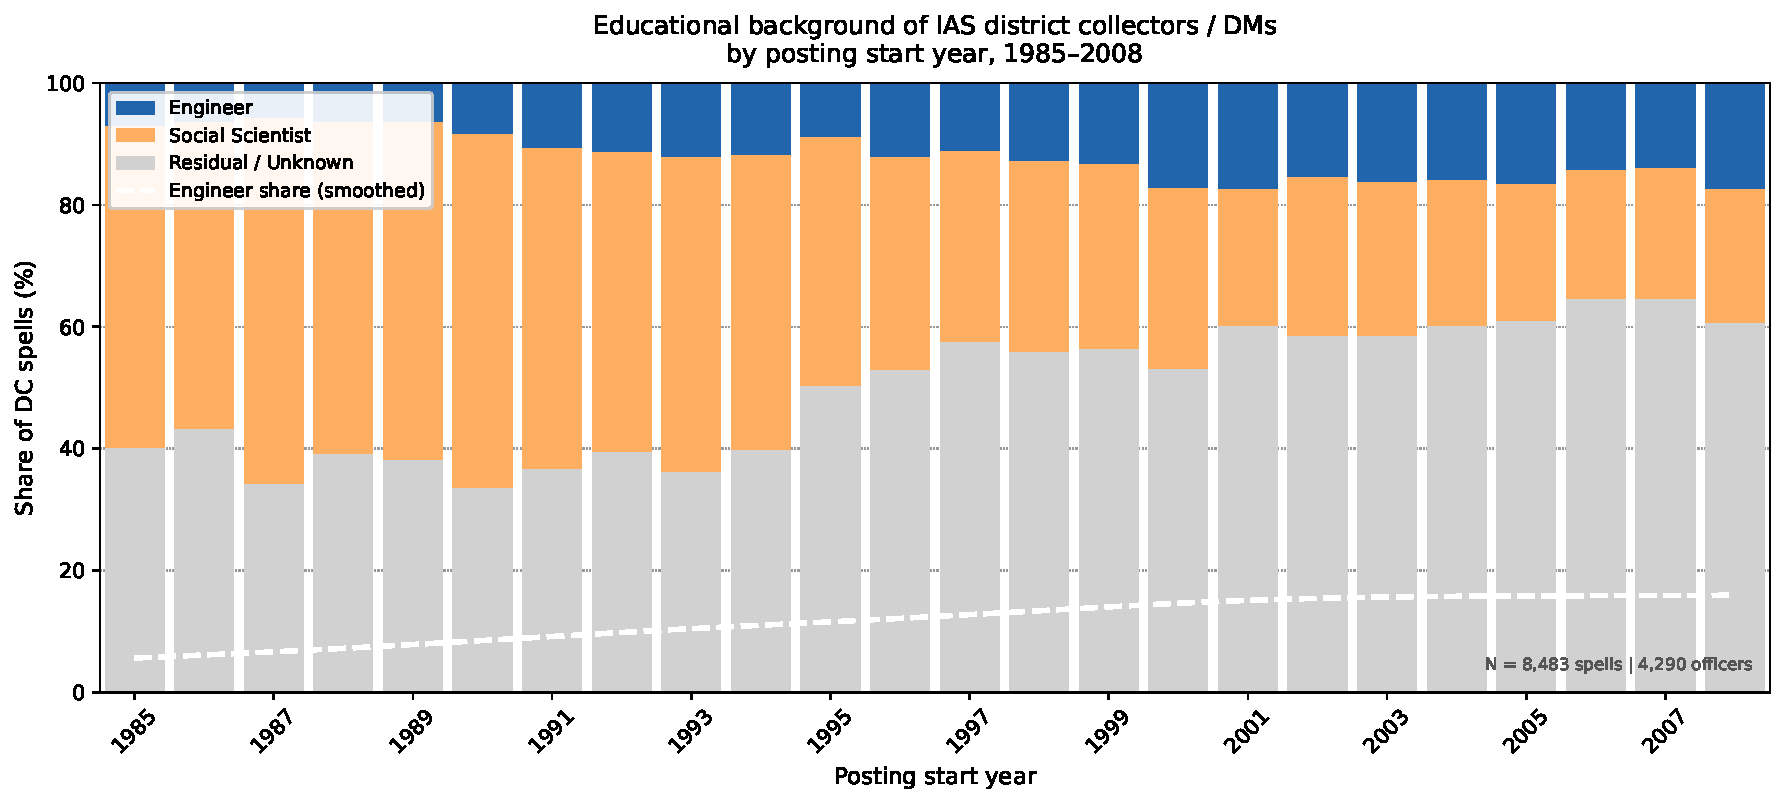
\includegraphics[width=0.95\linewidth]{engineer_share_over_time.pdf}
\end{figure}

\vspace{-0.5em}

{\small
Engineer share remains stable at roughly 7--12\% throughout the sample period. Social scientists account for 45--55\% of classified spells. Variation across time and states provides identifying variation in officer education type.
}

\end{column}
\end{columns}

\end{frame}

% ===============================================================
\section{Model}
% ===============================================================

\begin{frame}{Comparative Advantage in Program Delivery}

\textbf{Setup:} Officer $i$ of education type $\tau \in \{T, S, R\}$ produces output in program $k \in \{\text{infrastructure}, \text{welfare}\}$:

$$Y_{idt} = \eta(\tau_i,\, k_d) + \alpha_d + \lambda_{st} + \varepsilon_{idt}$$

where $\eta(\tau, k)$ is the implementation efficiency of type $\tau$ on program $k$.

\bigskip

\textbf{Predictions:}
\begin{itemize}
    \item[\textbf{P1}] $\eta(T, \text{infra}) > \eta(S, \text{infra})$: engineer advantage on infrastructure programs
    \item[\textbf{P2}] $\eta(S, \text{welfare}) > \eta(T, \text{welfare})$: social scientist advantage on welfare programs
    \item[\textbf{P3}] Engineer advantage increasing in district infrastructure program intensity
\end{itemize}

\bigskip


\end{frame}

% -------------------------------------------------------
\begin{frame}{Estimating Equation}

$$Y_{dt} = \beta_1 \cdot \text{Engineer}_{it} + \beta_2 \cdot \text{Residual}_{it} + \gamma X_{dt} + \alpha_d + \lambda_{st} + \varepsilon_{dt}$$

\medskip

\begin{itemize}
    \item $Y_{dt}$: outcome in district $d$, year $t$
    \item Social Scientist is the omitted baseline throughout
    \item $\beta_1$: engineer effect relative to social scientist
    \item $\alpha_d$: district fixed effects; $\lambda_{st}$: state $\times$ year fixed effects
    \item $X_{dt}$: officer tenure, seniority at posting, election year indicator
    \item Standard errors clustered at district
\end{itemize}

\bigskip

P1 predicts $\beta_1 > 0$ on infrastructure outcomes. P2 predicts $\beta_1 < 0$ on welfare outcomes.

\end{frame}

% -------------------------------------------------------
% CHANGE 2: Replaced "The Priority Queue" content; renamed frame
\begin{frame}{Identification via the Seniority Queue}

\begin{block}{Assignment Rule}
\[
i^*(d,t) = \arg\max_{i \in \mathcal{A}_{st}} r_i, \qquad
\mathcal{A}_{st} = \{i \in \mathcal{I}_s : a_{it} = 1\}
\]
\end{block}
\begin{itemize}\setlength\itemsep{4pt}
  \item Priority $r_i$ fixed at IAS entry --- independent of district characteristics
  \item Education type $e_i$ does not appear in the assignment rule
  \item Availability $a_{it}$ depends on state-wide rotation history, not district $d$
\end{itemize}

\bigskip

\begin{block}{Key Independence Result}
\[
e_{i^*(d,t)} \;\perp\; \mathbf{X}_d \;\Big|\; r_{i^*(d,t)},\, \mathcal{A}_{st}
\]
\end{block}
\begin{itemize}\setlength\itemsep{4pt}
  \item Education of assigned officer independent of district characteristics
  \item Verified empirically: joint $F = 0.89$,\; $p = 0.470$ (Table 1, Panel B)
\end{itemize}

\bigskip

\begin{block}{Instrument}
\[
Z_{it} = \mathrm{OppositionVictory}_{st} \times \mathrm{CadreQueuePct}_{it}
\]
\end{block}
\begin{itemize}\setlength\itemsep{4pt}
  \item First stage $F = 6.94$; instrument significant ($p = 0.018$)
  \item IV/OLS $= 0.94$ for roads: strategic assignment bias empirically small
  \item Sparse opposition-turnover events (20\% of sample) limit power ---
        longer panel would restore $F > 10$
\end{itemize}

\end{frame}

% CHANGE 3: Deleted "Identification: Empirical Support from the Literature" frame

% -------------------------------------------------------
\begin{frame}{Matched Analysis Sample}

\textbf{Merge:} IAS DC spells $\xrightarrow{\text{fuzzy name match}}$ district crosswalk $\xrightarrow{\text{pc11 ID}}$ panel outcomes

\bigskip

{\small
\begin{tabular}{lr}
\toprule
Total DC spell-years, 1985--2008 & 8,494 \\
Matched to Census 2011 district ID & 5,612 \ (66.1\%) \\
Within panel window, 1994--2013 & 5,670 \\
Matched to outcome row & 3,836 \ (67.7\% of in-panel spells) \\
\midrule
\multicolumn{2}{l}{\textit{Analysis sample (classified officers only)}} \\
Spell-years & 1,887 \\
Unique DC spells & 3,355 \\
Districts & 422 of 640 \ (66\%) \\
Years & 1994--2008 \\
\bottomrule
\end{tabular}
}

\bigskip

{\small Unmatched: blank office field (553 spells), department-level postings, or districts absent from crosswalk. Unclassified education (N.A.) excluded from regression sample; robustness to inclusion available on request.}

\end{frame}

% ===============================================================
\section{Results}
% ===============================================================

% CHANGE 5: Balance table via \input
\begin{frame}{Table 1: Balance}
\begin{center}
  \resizebox{0.90\linewidth}{!}{%
    \begin{minipage}{1.6\linewidth}
      \begin{table}[htbp]
\centering
\caption{Summary Statistics}
\label{tab:summary}
\textbf{Panel A: Officer characteristics}\\[4pt]
\begin{tabular}{lrrrr}
\toprule
Group & $N$ spells & Tenure (mo.) & Allot.\ year & \% Female \\
\midrule
Engineer         & 578   & 17.7 & 1992.6 &  4.2 \\
Social Scientist & 1,114 & 15.8 & 1990.5 & 13.6 \\
Residual         & 698   & 17.1 & 1990.8 & 10.2 \\
\bottomrule
\end{tabular}
\\[10pt]
\textbf{Panel B: District characteristics (pre-treatment Census values)}\\[4pt]
\begin{tabular}{lcccc}
\toprule
Characteristic      & Engineer & Soc.\ Sci. & Difference & $p$-value \\
\midrule
SC share            & 0.156 & 0.159 & $-$0.002  & 0.534 \\
ST share            & 0.137 & 0.120 & $+$0.018$^{*}$ & 0.084 \\
Literacy rate       & 0.525 & 0.532 & $-$0.007  & 0.260 \\
Population ('000)   & 1,855 & 1,940 & $-$85     & 0.355 \\
\midrule
Joint $F$-test      &       &       & 0.89      & 0.470 \\
\bottomrule
\end{tabular}
\par\vspace{4pt}
{\footnotesize Panel A: spell-year means. Panel B: district-level means from Census 2001.
Difference = Engineer $-$ Social Scientist. $^{*}p<0.10$, $^{**}p<0.05$, $^{***}p<0.01$.}
\end{table}

    \end{minipage}}
\end{center}
\end{frame}

% CHANGE 5: Infrastructure table via \input
\begin{frame}{Table 3: Infrastructure Outcomes}
\begin{center}
  \resizebox{\linewidth}{!}{%
    \begin{minipage}{1.85\linewidth}
      \begin{table}[htbp]
\centering
\caption{Effect of DC Education on Infrastructure Outcomes}
\label{tab:infrastructure}
\begin{tabular}{lcccccc}
\toprule
 & \multicolumn{3}{c}{Panel A: Nightlights per capita, 1994--2008} & \multicolumn{3}{c}{Panel B: Road completion rate, 2001--2008} \\
\cmidrule(lr){2-4}\cmidrule(lr){5-7}
 & (1) & (2) & (3) & (4) & (5) & (6) \\
\midrule
Engineer & -0.0007 & -0.0007 & -0.0010 & 0.0284 & 0.0233 & 0.0158 \\
       & (0.0008) & (0.0008) & (0.0008) & (0.0402) & (0.0411) & (0.0245) \\
\addlinespace
Residual & 0.0002 & 0.0004 & -0.0000 & 0.0007 & 0.0196 & 0.0412 \\
       & (0.0003) & (0.0004) & (0.0005) & (0.0379) & (0.0387) & (0.0268) \\
\addlinespace
\midrule
District FE          & \checkmark & \checkmark & \checkmark & \checkmark & \checkmark & \checkmark \\
Year FE              & \checkmark & \checkmark &  & \checkmark & \checkmark &  \\
State$\times$Year FE &  &  & \checkmark &  &  & \checkmark \\
Controls             &  & \checkmark & \checkmark &  & \checkmark & \checkmark \\
\midrule
$N$           & 2,390 & 2,274 & 2,274 & 596 & 586 & 586 \\
$R^2$         & 0.001 & 0.002 & 0.406 & 0.004 & 0.034 & 0.498 \\
Control mean  & 0.019 & 0.019 & 0.019 & 0.369 & 0.369 & 0.369 \\
\bottomrule
\end{tabular}
\par\vspace{4pt}{\footnotesize
Baseline: Social Scientist DCs. Panel A: DMSP light / population. Panel B: roads completed / total road length (km), 2001--2008.
Controls: tenure, allotment year, incumbent win. SE clustered at district. $^{*}p<0.10$, $^{**}p<0.05$, $^{***}p<0.01$.}
\end{table}
    \end{minipage}}
\end{center}
\vspace{2pt}
{\footnotesize \color{gray}
Engineer effect on roads positive across all specs; switches on with PMGSY (2001).
Nightlights near zero --- consistent with comparative advantage averaging across program types.}
\end{frame}

% CHANGE 5: Welfare table via \input
\begin{frame}{Table 4: Employment per Capita}
\begin{center}
  \resizebox{0.72\linewidth}{!}{%
    \begin{minipage}{1.6\linewidth}
      \begin{table}[htbp]
\centering
\caption{Effect of DC Education on Employment Outcomes (2006--2008)}
\label{tab:welfare}
\begin{tabular}{lccc}
\toprule
 & \multicolumn{3}{c}{Employment per capita (ec\_emp\_all / tot\_p)} \\
\cmidrule(lr){2-4}
 & (1) & (2) & (3) \\
\midrule
Engineer & 0.100*** & -0.000 & -0.000** \\
       & (0.015) & (0.000) & (0.000) \\
\addlinespace
Residual & 0.124*** & -0.000 & -0.000 \\
       & (0.017) & (0.000) & (0.000) \\
\addlinespace
\midrule
District FE    & \checkmark & \checkmark & \checkmark \\
Year FE        & \checkmark & \checkmark &  \\
State$\times$Year FE &  &  & \checkmark \\
Controls       &  & \checkmark & \checkmark \\
\midrule
$N$          & 438 & 433 & 433 \\
Within $R^2$ & ---   & 0.000 & 0.000 \\
Control mean & 0.076 & 0.076 & 0.076 \\
\bottomrule
\end{tabular}
\par\vspace{4pt}{\footnotesize
Sample: 2006--2008 (post-NREGA). Baseline: Social Scientist. Controls: tenure, allotment year, incumbent win.
SE clustered at district. $^{*}p<0.10$, $^{**}p<0.05$, $^{***}p<0.01$.}
\end{table}
    \end{minipage}}
\end{center}
\vspace{4pt}
{\footnotesize \color{gray}
Engineer coefficient negative in preferred spec (Spec 3, $p = 0.031$). Sign reversal rules out generic ability story.}
\end{frame}

% -------------------------------------------------------
\begin{frame}{Main Results: Coefficient Plot}
\begin{center}
  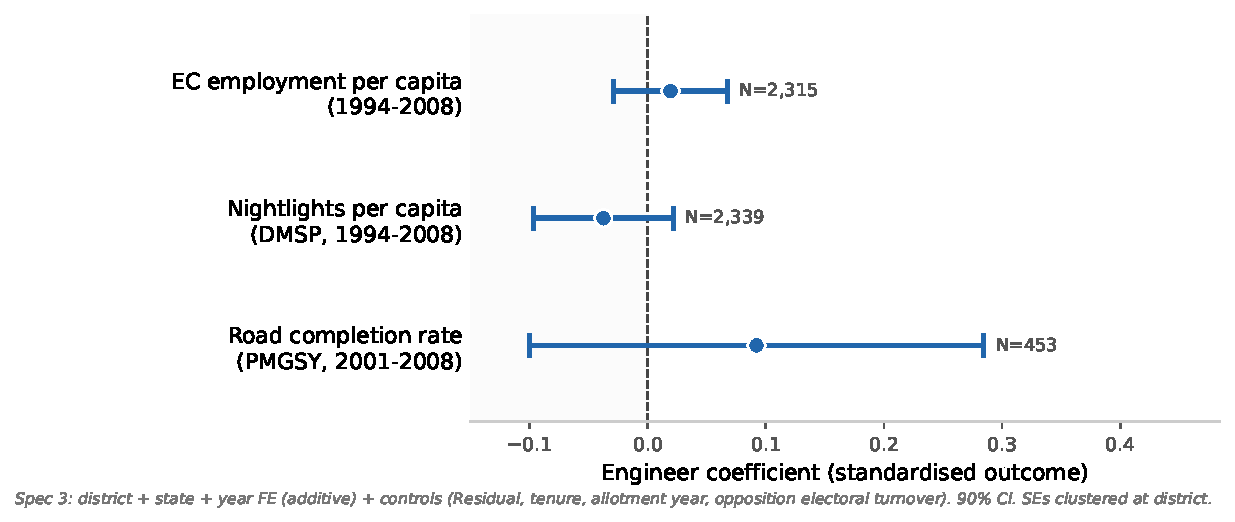
\includegraphics[width=0.88\textwidth]{coeff_plot_presentation.pdf}
\end{center}
\vspace{-4pt}
{\footnotesize \color{iasgray}
Engineer coefficient relative to Social Scientist (Spec 3: district FE + state$\times$year FE + controls).
Outcomes standardised to mean 0, SD 1. 90\% confidence intervals.
\textbf{Sign reversal rules out a generic-ability story.}}
\end{frame}

% -------------------------------------------------------
\begin{frame}{Summary of Estimates}

\textbf{Engineer coefficient ($\hat\beta_1$) relative to Social Scientist baseline, preferred specification (Spec 3):}

\bigskip

{\small
\begin{tabular}{lcc}
\toprule
\textbf{Outcome} & $\hat{\beta}_1$ & $p$-value \\
\midrule
Road completion rate       & $+$0.022       & 0.364 \\
Nightlights per capita     & $\approx 0.000$ & 0.921 \\
Non-farm employment p.c.   & $-$0.000$^{**}$ & 0.031 \\
\bottomrule
\end{tabular}
}

\bigskip

Engineer DCs show positive coefficients on infrastructure and negative on welfare-adjacent outcomes relative to Social Scientist DCs --- directionally consistent with P1 and P2 across all specifications.

\bigskip

A generic ability story predicts $\hat\beta_1 > 0$ uniformly. Sign reversal across program types is inconsistent with that hypothesis.

{\footnotesize Nightlights null consistent with comparative advantage: aggregate satellite luminosity averages infrastructure and welfare effects, which attenuate toward zero under P1 and P2.}

\end{frame}

% CHANGE 5: Instrument validation slide (new)
\begin{frame}{Instrument Validation}
  \begin{center}
    \resizebox{0.80\linewidth}{!}{%
      \begin{minipage}{1.6\linewidth}
        \begin{table}[htbp]
\centering
\caption{OLS vs 2SLS: Effect of Engineer DC on Infrastructure Outcomes}
\label{tab:iv_main_v2}
\begin{tabular}{lcccc}
\hline\hline
 & \multicolumn{2}{c}{Road completion rate} & \multicolumn{2}{c}{Nightlights per capita} \\
\cmidrule(lr){2-3}\cmidrule(lr){4-5}
 & OLS & 2SLS & OLS & 2SLS \\
 & (1) & (2) & (3) & (4) \\
\hline
Engineer & 0.0281 & 0.0265 & -0.0008 & 0.0386 \\
          & (0.0249) & (0.1993) & (0.0007) & (0.0390) \\[4pt]
First-stage $F$ & --- & 6.94~$\times$ & --- & 6.18~$\times$ \\
Observations & 453 & 453 & 2,339 & 2,339 \\
\hline
District FE  & \checkmark & \checkmark & \checkmark & \checkmark \\
Year FE      & \checkmark & \checkmark & \checkmark & \checkmark \\
\hline\hline
\multicolumn{5}{p{0.90\textwidth}}{\footnotesize
\textit{Notes:} Baseline category: SocialScientist.
Instrument (2SLS): Queue\_refined $=$ opposition\_turnover $\times$
cadre\_queue\_pct, where opposition\_turnover $=1$ when incoming
state government is from a different party than outgoing,
and cadre\_queue\_pct $\in[0,1]$ is officer's percentile position
in the cadre's seniority queue in that year (0 = most senior).
Cols (1)--(2): roads subsample, year $\geq 2001$.
Cols (3)--(4): full panel, 1994--2008.
Clustered SEs at district level. $\checkmark$: $F>10$; $\times$: $F\leq10$.
Stars: *** $p<0.01$, ** $p<0.05$, * $p<0.10$.}
\end{tabular}
\end{table}

      \end{minipage}}
  \end{center}
  \vspace{4pt}
  \begin{itemize}\setlength\itemsep{5pt}
    \item \textbf{First stage:} Queue\_refined $\to$ Engineer,
          $F = 6.94$ (roads), $F = 6.18$ (full panel)
    \item \textbf{IV/OLS ratio = 0.94} for roads:
          strategic assignment bias is empirically small
    \item \textbf{Why $F < 10$:} opposition-turnover years are sparse
          (20\,\% of observations) --- longer panel restores power
  \end{itemize}
\end{frame}

% CHANGE 5: Robustness table via \input
\begin{frame}{Robustness}
\begin{center}
  \resizebox{\linewidth}{!}{%
    \begin{minipage}{1.6\linewidth}
      \begin{table}[htbp]
\centering
\caption{Robustness Checks — Engineer Coefficient (Spec 2 baseline)}
\label{tab:robustness}
\begin{tabular}{lcccc}
\toprule
 & \shortstack{R1: tenure $\geq$\\ 6 mo.} & \shortstack{R2: 1994--2004} & \shortstack{R3: state cluster} & \shortstack{R4: pure-ID districts} \\
 & (1) & (2) & (3) & (4) \\
\midrule
\multicolumn{5}{l}{\textit{Panel A: Nightlights per capita}} \\
Engineer & 0.000 & -0.000 & -0.001 & -0.001 \\
         & (0.000) & (0.000) & (0.001) & (0.001) \\
$N$ & 1,933 & 1,687 & 2,274 & 2,068 \\
\addlinespace
\multicolumn{5}{l}{\textit{Panel B: Road completion rate}} \\
Engineer & 0.031 & 0.037 & 0.023 & 0.023 \\
         & (0.058) & (0.160) & (0.038) & (0.040) \\
$N$ & 481 & 244 & 586 & 515 \\
\addlinespace
\bottomrule
\end{tabular}
\par\vspace{4pt}{\footnotesize
All specs: district FE + year FE + controls. Baseline: Social Scientist.
R1: tenure $\geq$6 mo. R2: 1994--2004. R3: state clustering. R4: pure-ID districts.
$^{*}p<0.10$, $^{**}p<0.05$, $^{***}p<0.01$.}
\end{table}
    \end{minipage}}
\end{center}
\vspace{4pt}
{\footnotesize \color{gray}
Sign and magnitude stable across: short-tenure exclusion, pre-2005 sample, state-level clustering, pure-ID-district restriction.}
\end{frame}

% -------------------------------------------------------
% CHANGE 4: Restructured Next Steps bullets
\begin{frame}{Next Steps}

\begin{itemize}\setlength\itemsep{14pt}
  \item \textbf{Heterogeneity (P3)} ---
        Engineer $\times$ infrastructure-intensity interaction

  \item \textbf{NREGA MIS outcomes} ---
        direct program-specific welfare test

  \item \textbf{Extend panel to 2013} ---
        restores instrument power ($F > 10$ target)

  \item \textbf{Optimal allocation extension} ---
        two-stage mechanism: seniority determines eligibility,
        education determines assignment within tier
        {\small (Abdulkadiro\u{g}lu \& S\"onmez 2003;
        Roth \& Sotomayor 1990)}
\end{itemize}

\end{frame}

% ===============================================================
\section{Mechanism Design Extension}
% ===============================================================

\begin{frame}{The Optimal Matching Problem}

\begin{block}{Current Mechanism: Seniority Queue}
\[
i^*(d,t) = \arg\max_{i \in \mathcal{A}_{st}} r_i
\qquad \textcolor{iasred}{\text{[ignores match quality]}}
\]
\end{block}

\bigskip

\begin{block}{Optimal Two-Stage Mechanism}
\[
i^*(d,t) = \arg\max_{\substack{i \in \mathcal{A}_{st} \\ r_i \,\geq\, \bar{r}}}
\eta(e_i,\, \tau_d)
\qquad \textcolor{iasblue}{\text{[seniority then match quality]}}
\]
\end{block}

\begin{itemize}\setlength\itemsep{4pt}
  \item Stage 1: seniority threshold $\bar{r}$ preserves career incentives
  \item Stage 2: within eligible pool, assign engineer $\to$ infra district,
        social scientist $\to$ welfare district
  \item Stable in the sense of Roth \& Sotomayor (1990):
        no officer-district pair mutually prefers to deviate
\end{itemize}

\bigskip

\begin{block}{Why It Is Implementable Today}
\begin{itemize}\setlength\itemsep{3pt}
  \item State government observes $e_i$ --- education recorded at IAS entry
  \item State government observes $\tau_d$ --- program budget shares are public
  \item \textbf{Zero additional information required}
\end{itemize}
\end{block}

\vspace{4pt}
{\footnotesize \color{iasgray}
Quantifying aggregate welfare gain from reallocation:
$\Delta W = \sum_d \left[\eta(\hat e^*_d, \tau_d) - \eta(\tilde e_d, \tau_d)\right] \cdot \bar B_d$
where $\hat e^*_d$ is optimal assignment and $\tilde e_d$ is current assignment.
Even under imprecise $\hat\beta$, bootstrap CIs bound the welfare gain from above.}

\end{frame}

% -------------------------------------------------------
\begin{frame}{Conclusion}

\textbf{Question:} Does educational background of the District Collector affect public goods delivery across program types?

\bigskip

\textbf{Preliminary findings:}
\begin{itemize}
    \item Engineer and social scientist DCs posted to observationally equivalent districts: joint $F = 0.89$, $p = 0.470$
    \item Engineer DCs show positive coefficients on road completion rates relative to social scientist baseline across all specifications
    \item Engineer DCs show negative coefficients on non-farm employment per capita, significant at 5\% in preferred specification ($p = 0.031$)
    \item Pattern is directionally consistent with comparative advantage; inconsistent with a generic ability explanation
\end{itemize}

\bigskip

\textbf{Policy implication:} A posting rule incorporating educational background could improve program delivery at zero additional fiscal cost.

\bigskip

\end{frame}

\end{document}
